% openany makes chapters start on even pages too
\documentclass[openany, 12pt]{book}

% sets margins of text inside page to 1 inch
\usepackage[top=1in, bottom=1in, left=1in, right=1in]{geometry}

% this will indent the first paragraph in a chapter
\usepackage{indentfirst}

% to use href
\usepackage{hyperref}

% to use images
\usepackage{graphicx}
% where images are stored
\graphicspath{{images/}}

\title{
  Introduction to Fitness \\
  \vskip 0.5cm
  \small A Technical Book on Fitness}
\author{Mihail Dunaev}
% this will remove date
\date{}

\begin{document}
  \maketitle
  \tableofcontents

  \chapter{Introduction}
  
	I have no background in fitness or nutrition. In school I studied Computer Science and now I work as a Software Engineer. What made me get more 
	into fitness was my weight: I was fat. Multiple times in my life. First, growing up as a kid I was fat and I managed to lose the weight in 
	secondary school just by eating less. Second time I got fat was in university, just because I lacked any motivation to study for exams and would
	power my way through with food and energy drinks. After uni I found it much harder to lose weight than I previously knew. I would follow a lot 
	of diets (keto\footnote{\href{https://en.wikipedia.org/wiki/Ketogenic_diet}{Ketogenic Diet}}, food replacement like 
	soylent\footnote{\href{https://en.wikipedia.org/wiki/Soylent_(meal_replacement)}{Soylent}} or huel\footnote{\href{https://en.wikipedia.org/wiki/Huel}
	{Huel}}), sometimes going really low in calories intake, feeling like I have no energy and gaining the weight back on after ending the diet. I 
	needed a better solution to this: I decided to start going to the gym.
	
	I guess my goal was to build muscle and lose fat. I've always liked muscles as a kid, just never got the time to look into it and start
	working out. This was my chance. I had a lot of questions: how do I train? What do I eat? Are there other things I need to pay attention to?
	One solution would be to hire a personal trainer to help me achieve this goal. What stopped me from doing this is the way my brain works: I knew
	I would just be given a list of things to do without any explanation. I really like to understand how things work and I would end up being 
	disappointed. This is also a big part of my life by now, I definitely wanted to understand well how everything works. I started looking into fitness
	the same way I look into everything: start searching on google, looking at professional bodybuilders, what they say, does it make sense etc. 
	I feel that if you want to know a subject really well you should look for competitions related to that subject, and see what the people involved
	have to say about it. This is why I started following people that compete in bodybuilding shows, strongman competitions and so on. 	
	What bothered me was how poorly organised the fitness information I found was. I couldn't find a single place that could take me from 0 knowledge
	to getting started in a matter of few hours. I had to watch a lot of youtube videos, read a lot of articles and posts in fitness communities until
	things were clear in my head. Now that I know all this information I think it's possible to put it all in one place: this is the purpose of this 
	book, to get you started with your fitness journey, especially if your goal is to build muscles and lose fat. And as I understand, this is the case
	for	most people working out.
	
	I just want to stress out: there is nothing wrong with being fat. If you get really fat it is unhealthy and you'll end up with 
	health problems. However, the main reason I don't want to be fat is because I get anxiety from it. I feel like crap, especially if I take my shirt 
	off in public. Saying I don't care about it is just lying to myself and I try my best to not do that, just for my mental health. This anxiety is
	something I can't control so for me the only solution would be to stay in shape. Besides, I already said I like muscles, so becoming muscular would
	make me feel proud of myself.
	
	The book is structured in two parts: nutrition \& workout. There is a lot of information in here, you don't necessarily need to understand all of it
	to get going. That's why at the end I just added an example of everything I did to get in my current shape without extra explanations. I will try 
	my best to present information in an unbiased way, presenting what people think works and what not, what I tried on myself etc. If you think 
	something is wrong or don't agree with some of the information presented here, this is an open source book so feel free to submit a 
	PR!\footnote{\href{https://docs.github.com/en/free-pro-team@latest/github/collaborating-with-issues-and-pull-requests/about-pull-requests}
	{Pull Request}} At the end of the day I am a practical person, I only believe in results and what works in real life. I can say that the 
	information I describe in this book worked really well on me, as you can see in the picture below.
	
	\begin{figure}[h]
		\centering
		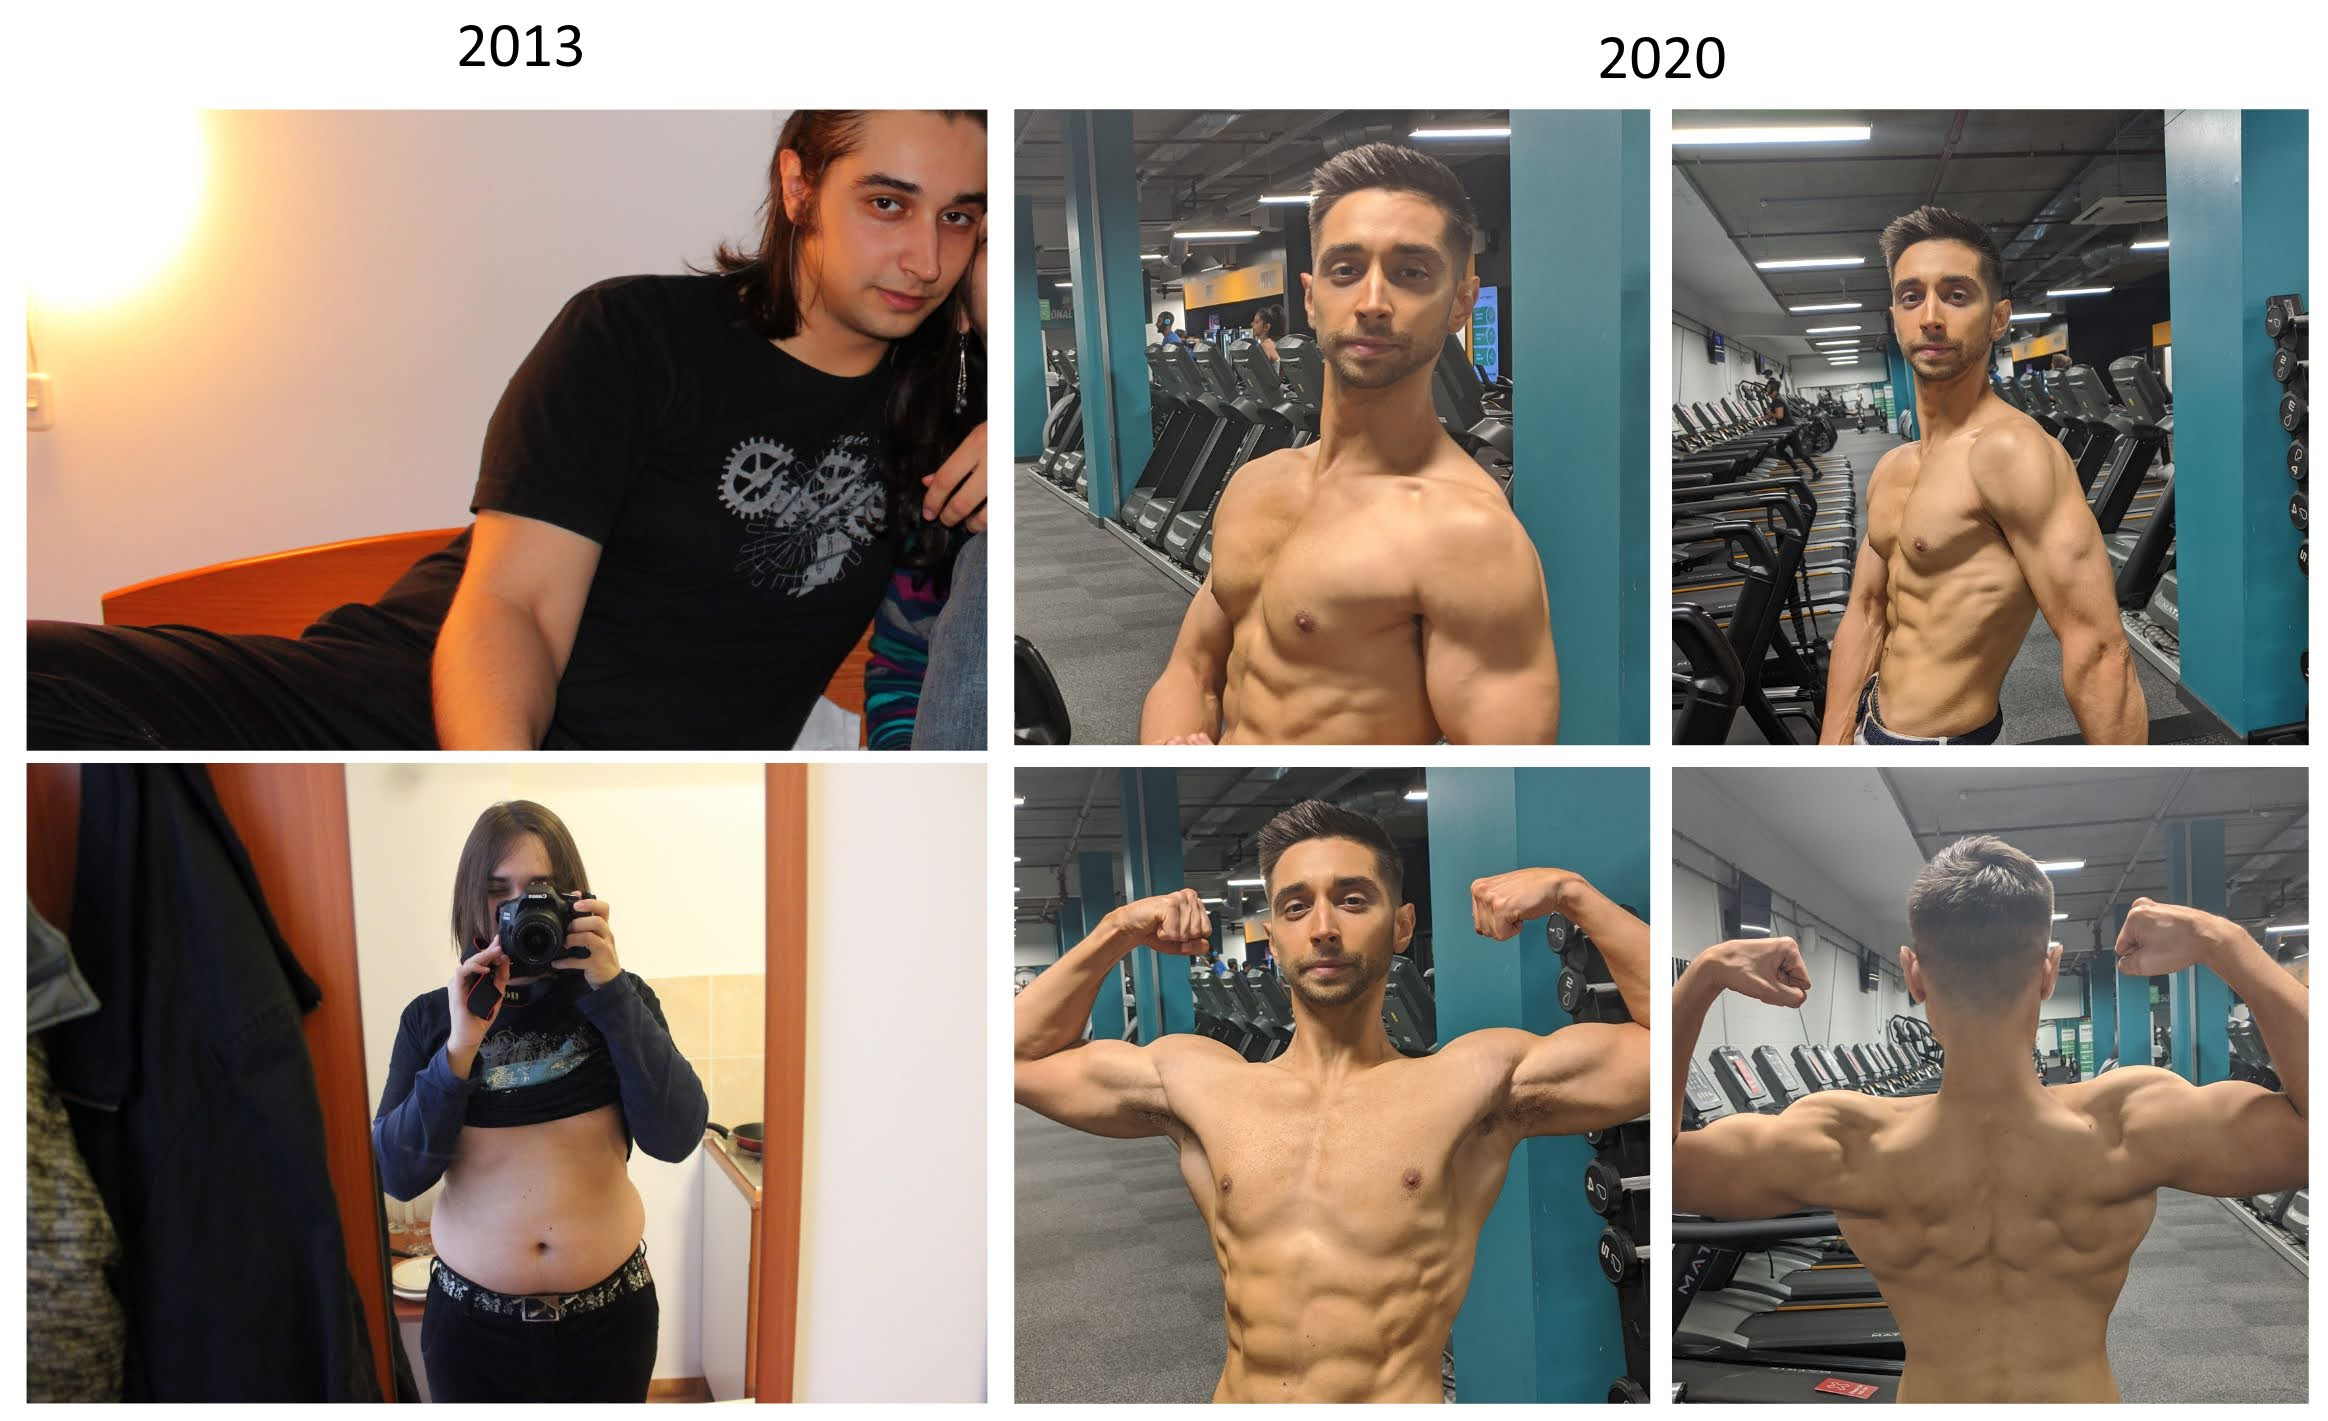
\includegraphics[scale=0.2]{transformation.jpg}
		\caption{From fat to muscular in 7 years: my lifelong struggle with being fat}
		\label{fig1}
	\end{figure}
	
\end{document}
